\documentclass[a4paper]{article}
\usepackage[pdftex]{graphicx}
\usepackage[utf8]{inputenc}
\usepackage{enumerate}
\usepackage{icomma}
\usepackage{amssymb}
\usepackage{tikz}
\usepackage{href-ul}
\hypersetup{
	colorlinks=true,
	linkcolor=blue,
	urlcolor=blue}
\usepackage{geometry}
\geometry{a4paper, top=15mm, left=15mm, right=15mm, bottom=15mm,
headsep=10mm, footskip=12mm}


\begin{document}
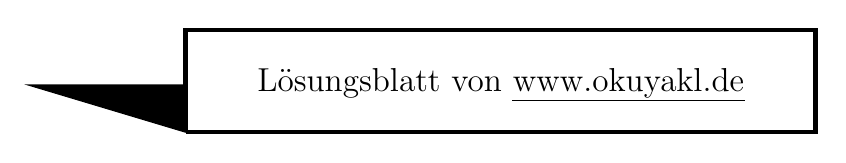
\begin{tikzpicture}(10,3)
	\draw[ultra thick](2,0) --(10,0) -- (10,1.3) --(2,1.3) -- (2,0);
	\draw[fill=black](2,0)-- (0,.6) -- (2,.6) -- (2,0);
	\node at (6,.6) {\large Lösungsblatt von \href{https://www.okuyakl.de}{www.okuyakl.de}};
\end{tikzpicture}
\vspace{0.5 cm}

\noindent{\bf Lösung}\\
\noindent{\bf Aufgabe 1.}\\
$$|\overrightarrow{PQ}|=6 \quad \Rightarrow \quad \overrightarrow{PQ}= 
\left(\begin{array}{c} 6 \\ 0 \\ 0 \end{array} \right)\qquad \Rightarrow \quad \textnormal{z.B.} \quad P(1|1|1); \quad Q(7|1|1)$$

\noindent{\bf Aufgabe 2.}\\
Die Vektoren müssen erstens senkrecht aufeinander stehen...
$$\overrightarrow{AB} \circ \overrightarrow{AD}= \quad
 \left( \begin{array}{c} {1}\\ {2}\\ {2} \end{array} \right) \circ 
   \left( \begin{array}{c} {2}\\ {1}\\ {-2} \end{array} \right) =2+2-4=0$$

$$\overrightarrow{AB} \circ \overrightarrow{AE}= \quad
\left( \begin{array}{c} {1}\\ {2}\\ {2} \end{array} \right) \circ 
 \left( \begin{array}{c} {2}\\ {-2}\\ {1} \end{array} \right)=2-4+2=0 $$

$$\overrightarrow{AD} \circ \overrightarrow{AE}= \quad
\left( \begin{array}{c} {2}\\ {1}\\ {-2} \end{array} \right) \circ
 \left( \begin{array}{c} {2}\\ {-2}\\ {1} \end{array} \right)=4-2-2=0$$
 
...und zweitens  müssen sie gleich lang sein:

$$|\overrightarrow{AB}|=\sqrt{1+2^2+2^2} = 3 \qquad |\overrightarrow{AE}|=\sqrt{2^2+(-2)^2+1} = 3 \qquad |\overrightarrow{AD}|=\sqrt{2^2+1+(-2)^2} = 3 ;$$
 
\noindent{\bf Aufgabe 3. a)}\\
\begin{minipage}{0.3\textwidth}
\setlength{\unitlength}{0.5 cm}
\begin{picture}(8,6)
\put(1,1){\vector(1,0){5}}
\put(1,1){\vector(1,2){1.5}}
\put(2.5,4){\vector(1,0){5}}
\put(6,1){\vector(1,2){1.5}}
\put(0.5,0.5){O}
\put(6.2,0.5){B}
\put(7.8,4){C}
\put(2,4){D}
\end{picture}
\end{minipage}
\begin{minipage}{0.7\textwidth}
Es gilt die Vektorkette:
$$\overrightarrow{OC}=\overrightarrow{OB}+\overrightarrow{BC}$$
Mit $\overrightarrow{BC}=\overrightarrow{OD}$ folgt:
$$\overrightarrow{OC}=\overrightarrow{OB}+\overrightarrow{OD}= 
\left( \begin{array}{c} {-3}\\ {4}\\ {0} \end{array} \right) +
\left( \begin{array}{c} {-2}\\ {1}\\ {2} \end{array} \right) =
\left( \begin{array}{c} {-5}\\ {5}\\ {2} \end{array} \right) \Rightarrow \quad
C(-5|5|2)$$
\end{minipage}
\noindent{\bf Aufgabe 3. b)}\\
Der Inhalt der Grundfläche $G$ ist gleich dem Betrag des Vektorproduktes:
$$G=|\overrightarrow{OB} \times \overrightarrow{OD}|=
\left| \left( \begin{array}{c} {-3}\\ {4}\\ {0} \end{array} \right) \times
\left( \begin{array}{c} {-2}\\ {1}\\ {2} \end{array} \right)\right| =
\left| \left( \begin{array}{c} {8}\\ {6}\\ {5} \end{array} \right)\right|=\sqrt{8^2+6^2+5^2}=5\sqrt{5}$$
\noindent{\bf Aufgabe 3. c)}\\
\begin{minipage}{0.3\textwidth}
\includegraphics[width=5 cm]{pyvec337}
\end{minipage}
\begin{minipage}{0.7\textwidth}
Der Mittelpunkt der Grundfläche $M_G$ hat die Koordinaten: $$\overrightarrow{OM_G} = {1 \over 2} \cdot(\vec{0}+\overrightarrow{OC})={1 \over 2}\left( \begin{array}{c} {-5}\\ {5}\\ {2} \end{array} \right)=\left( \begin{array}{c} {-2,5}\\ {2,5}\\ {1} \end{array} \right)\Rightarrow \quad 
M_G(-2,5|2,5|1)$$ 
Der Vektor$\overrightarrow{M_GS}$, der die Spitze $S$ mit dem Mittelpunkt verbindet, steht senkrecht auf der Grundfläche, verläuft also in Richtung des Vektors 
$\overrightarrow{OB} \times \overrightarrow{OD}= \left( \begin{array}{c} {8}\\ {6}\\ {5} \end{array} \right)$. Da dieser schon die Länge $5 \sqrt{5}$ hat, können wir ihn gleich als $$\overrightarrow{M_GS}$$ übernehmen.
\end{minipage}
Für den Ortsvektor der Spitze gilt dann die Vektorkette:
$$\overrightarrow{OS}=\overrightarrow{OM_G}+\overrightarrow{M_GS}=\left( \begin{array}{c} {-2,5}\\ {2,5}\\ {1} \end{array} \right)+ \left( \begin{array}{c} {8}\\ {6}\\ {5} \end{array} \right) 
=\left( \begin{array}{c} {5,5}\\ {8,5}\\ {6} \end{array} \right)$$
\noindent{\bf Aufgabe 3. d)}\\
Der Punkt $N$ auf der x-Achse hat die gleiche $x_2$-Koordinate wie Punkt $D$, also ist $N(0|1|0)$.
Der Radiusvektor des Kreises ist mit seinem Betrag:
$$\overrightarrow{ND}=\left( \begin{array}{c} {-2}\\ {1}\\ {2} \end{array} \right)-\left( \begin{array}{c} {0}\\ {1}\\ {0} \end{array} \right)=
\left( \begin{array}{c} {-2}\\ {0}\\ {2} \end{array} \right) \qquad |\overrightarrow{ND}|= \sqrt{4+4}=2\sqrt{2}$$    
\newpage

\begin{minipage}{0.4\textwidth}
\noindent{\bf Aufgabe 4. a)}\\
Die Punkte $A$ und $D$ liegen beide in der $x_1x_3$-Ebene.\\
\includegraphics[width=7 cm]{eder337}
\end{minipage}
\hspace{0.5 cm}
\begin{minipage}{0.5\textwidth} 
\noindent{\bf Aufgabe 4. b)}\\
Ein reguläres Tetraeder besteht aus vier gleichseitigen Dreiecken. Zu zeigen ist, dass gilt:
$$|\overrightarrow{AB}|=|\overrightarrow{AC}|=|\overrightarrow{AD}|$$
$$|\overrightarrow{AB}|=\left|\left( \begin{array}{c} {-4}\\ {5}\\ {-3} \end{array} \right)\right|=
\sqrt{16+25+9}=\underline{5\sqrt{2}}$$
$$|\overrightarrow{AC}|=\left|\left( \begin{array}{c} {-3}\\ {5}\\ {4} \end{array} \right)\right|=
\sqrt{9+25+16}=\underline{5\sqrt{2}}$$
$$|\overrightarrow{AD}|=\left|\left( \begin{array}{c} {-7}\\ {0}\\ {1} \end{array} \right)\right|=
\sqrt{49+1}=\underline{5\sqrt{2}}$$
\end{minipage}\\
Weiter muss gelten, dass der Winkel zwischen den genannten Vektoren $60^\circ$ beträgt:
$$\angle(\overrightarrow{AB},\overrightarrow{AC})=\cos^{-1}{\left( \begin{array}{c} {-4}\\ {5}\\ {-3} \end{array} \right) \circ \left( \begin{array}{c} {-3}\\ {5}\\ {4} \end{array} \right) \over \sqrt{50} \cdot \sqrt{50}}=\cos^{-1}{12+25-12 \over 50}=\cos^{-1}{1 \over 2} = 60^\circ$$
$$\angle(\overrightarrow{AB},\overrightarrow{AD})=\cos^{-1}{\left( \begin{array}{c} {-4}\\ {5}\\ {-3} \end{array} \right) \circ \left( \begin{array}{c} {-7}\\ {0}\\ {1} \end{array} \right) \over \sqrt{50} \cdot \sqrt{50}}=\cos^{-1}{28-3 \over 50}=\cos^{-1}{1 \over 2} = 60^\circ$$
\noindent{\bf Aufgabe 4. c)}\\
Der Mittelpunkt $M_T$ des Tetraeders ist:
$$\overrightarrow{OM_T}={1 \over 4}\cdot(\overrightarrow{OA}+\overrightarrow{OB}+\overrightarrow{OC}+\overrightarrow{OD})={1 \over 4}\cdot \left[ 
\left( \begin{array}{c} {4}\\ {0}\\ {3} \end{array} \right)+
\left( \begin{array}{c} {0}\\ {5}\\ {0} \end{array} \right)+
\left( \begin{array}{c} {1}\\ {5}\\ {7} \end{array} \right)+
\left( \begin{array}{c} {-3}\\ {0}\\ {4} \end{array} \right)\right]=
\left( \begin{array}{c} {0,5}\\ {2,5}\\ {3,5} \end{array} \right)  
\Rightarrow \quad M_T(0,5|2,5|3,5)$$
Wir bilden die Vektoren $\overrightarrow{M_TA}$ und $\overrightarrow{M_TB}$:
$$\overrightarrow{M_TA}=\left( \begin{array}{c} {3,5}\\ {-2,5}\\ {-0,5} \end{array} \right) \qquad
  \overrightarrow{M_TB}=\left( \begin{array}{c} {-0,5}\\ {2,5}\\ {-3,5} \end{array} \right) $$
Der Winkel zwischen diesen beiden Vektoren ist:
$$\cos{\varphi}=\frac{ \left( \begin{array}{c} {3,5}\\ {-2,5}\\ {-0,5} \end{array} \right) \circ
\left( \begin{array}{c} {-0,5}\\ {2,5}\\ {-3,5} \end{array} \right) }{\sqrt{3,5^2+2,5^2+0,5^2}\cdot \sqrt{0,5^2+2,5^2+3,5^2}}=\frac{-6,25}{18,75}=-{1 \over 3} \Rightarrow 
\qquad \varphi \approx 109,5^\circ$$
\noindent{\bf Aufgabe 4. d)}\\
Der Oberflächeninhalt ist viermal die Dreiecksfläche:
$$O_T=4\cdot {1 \over 2} |\overrightarrow{AB} \times \overrightarrow{AD}|=2\cdot
\left| \left( \begin{array}{c} {-4}\\ {5}\\ {-3} \end{array} \right) \times
\left( \begin{array}{c} {-7}\\ {0}\\ {1} \end{array} \right)\right| = 2 \cdot
\left| \left( \begin{array}{c} {5}\\ {25}\\ {35} \end{array} \right)\right|=2\cdot
\sqrt{5^2+25^2+35^2}=50\sqrt{3} \approx 86,60\, {\rm FE}$$
Das Volumen errechnet sich mit dem Spatprodukt:
$$V_T={1 \over 6}(\overrightarrow{AB}\times \overrightarrow{AD})\circ \overrightarrow{AC}={1 \over 6}
\left( \begin{array}{c} {5}\\ {25}\\ {35} \end{array} \right)\circ \left( \begin{array}{c} {-3}\\ {5}\\ {4} \end{array} \right)={250 \over 6} \approx 41,7 \, {\rm VE} $$
\newpage
\noindent{\bf Aufgabe 4. e)}\\
\begin{minipage}{0.7\textwidth}
Das Dreieck $ABC$ wird durch zentrische Streckung mit dem Zentrum $A$ und dem Streckungsfaktor 
$k={1 \over 2}$ auf das Dreieck $AM_1M_2$ abgebildet. Alle Abmessungen des kleinen Dreiecks sind  dann halb so groß wie die des ursprünglichen Dreiecks, der Flächeninhalt ist dann 
$$A_d=\left({1 \over 2}\right)^2 \cdot A_D={1 \over 4} \cdot A_D= 5,41 \, FE$$ 
Der Rauminhalt des kleinen Tetraeders ist 
$$V_t=\left({1 \over 2}\right)^3\cdot V_T={1\over 8}\cdot V_T ={125\over 24}\approx 5,21 \, {\rm VE}$$
\end{minipage}
\begin{minipage}{0.3\textwidth}
\setlength{\unitlength}{0.8 cm}
\begin{picture}(7,7)
\put(1,3){\line(2,-1){5}}
\put(1,3){\line(2,1){5}}
\put(1,3){\line(2,-1){5}}
\put(3.5,4.25){\line(0,-1){2.5}}
\put(6,5.5){\line(0,-1){5}}
\put(0.3,3.5){$A$}
\put(3.1,1.1){$M_1$}
\put(3.1,4.7){$M_2$}
\put(6.3,0.5){$B$}
\put(6.3,5.6){$C$}
\end{picture}
\end{minipage}

\noindent{\bf Aufgabe 4. f)}\\
Das Volumen des Pyramidenstumpfes ist: 
$$V_{S}=V_T-V_t= {250 \over 6} \cdot \left( 1 - {1\over 8} \right) \approx 36,46 \,{\rm VE} $$
Der Oberflächeninhalt des Stumpfes ist gleich dem des großen Tetraeders minus drei kleine Dreiecke plus ein kleines Dreieck als Schnittfläche:
$$O_S=O_T-3\cdot A_d + A_d = O_T - 2 A_d= 50\sqrt{3} -2\cdot 5,41 = 75,78 \, {\rm FE}$$

\noindent{\bf Aufgabe 5.}\\
\begin{minipage}{0.3\textwidth}
\setlength{\unitlength}{0.5 cm}
\begin{picture}(10,8)
\put(1,1){\includegraphics[width=4 cm]{parl337}}
\put(4,1){$\vec{a}$}
\put(1.5,5){$\vec{b}$}
\put(3,2.5){$\vec{a}+\vec{b}$}
\put(3.5,6.3){$\vec{a}-\vec{b}$}
\end{picture}
\end{minipage}
\begin{minipage}{0.7\textwidth}
Betrachtet wird ein Parallelogramm, welches von den Vektoren $\vec{a}$ und $\vec{b}$ aufge\-spannt wird. Dann sind die Diagolalen $\vec{a}+\vec{b}$ und $\vec{a}-\vec{b}$. Die Quadrate über die Vektoren haben den Flächeninhalt $|\vec{v}|^2 = \vec{v}\circ \vec{v}$. Es gilt dann für die Fläche $A_Q$ der Diagonalenquadrate:
$$A_Q=(\vec{a}+\vec{b})\circ (\vec{a}+\vec{b}) + (\vec{a}-\vec{b})\circ (\vec{a}-\vec{b})=
\vec{a}^2 +2\cdot \vec{a}\circ \vec{b} + \vec{b^2} + \vec{a}^2 -2\cdot \vec{a}\circ \vec{b} +
\vec{b}^2= 2\vec{a}^2+2\vec{b}^2$$
Dies entspricht genau dem Flächeninhalt der Quadrate über den zwei $\vec{a}$ und den zwei $\vec{b}$ Vektoren.
\end{minipage}


\noindent{\bf Aufgabe 6. a)}\\
Die Koordinaten der Punkte in der $x_1x_2$-Ebene lauten:
$$A(2|-3|0) \qquad B(1|4|0) \qquad C(-3|-4|0)$$
\noindent{\bf Aufgabe 6. b)}\\
Die Flächeninhalte liefert das Vektorprodukt. Ursprüngliches Dreieck:
$$A_D={1\over 2}\cdot |\overrightarrow{AB} \times \overrightarrow{AC}|={1\over 2}\cdot 
\left| \left( \begin{array}{c} {-1}\\ {7}\\ {2} \end{array} \right) \times
\left( \begin{array}{c} {-5}\\ {1}\\ {-2} \end{array} \right)\right|={1\over 2}
\left| \left( \begin{array}{c} {-16}\\ {-12}\\ {34} \end{array} \right) \right|
={1\over 2}\sqrt{16^2+12^2+34^2}\approx 19,72 \, {\rm FE}$$
Projiziertes Dreieck:
$$A_D'={1\over 2}\cdot |\overrightarrow{A'B'} \times \overrightarrow{A'C'}|={1\over 2}\cdot 
\left| \left( \begin{array}{c} {-1}\\ {7}\\ {0} \end{array} \right) \times
\left( \begin{array}{c} {-5}\\ {1}\\ {0} \end{array} \right)\right|={1\over 2}
\left| \left( \begin{array}{c} {0}\\ {0}\\ {34} \end{array} \right) \right|
= {1\over 2} \cdot 34 =17\, {\rm FE}$$
Der Flächeninhalt des projizierten Dreiecks ist um 
$$(1-{17 \over 19,72})\cdot 100\% = 13,8\%$$ 
kleiner als der des ursprünglichen.

\noindent {\bf Aufgabe 7. a)}\\
Der Punkt $A$ auf der Kugel erfüllt die Vektorgleichung:
$$
\renewcommand{\arraystretch}{1.5}
\begin{array}{rcll}
[\overrightarrow A -\overrightarrow M]^2 &=& r^2 &(I)\\ 
\\
\left[ \left( \begin{array}{c} 8 \\ 2 \\ 5 \end{array}\right)-
\left( \begin{array}{c} 2 \\ -1 \\ 7 \end{array}\right)\right]^2&=& \\
6^2 + 3^2 + (-2)^2 &=& 49
\end{array}
$$
Die Kugel hat also den Radius $r=\sqrt{49}=7$. Wir setzen nun den Punkt $B_k$ in 
(I) ein:
$$
\renewcommand{\arraystretch}{1.5}
\begin{array}{rcll}
[\overrightarrow B_k -\overrightarrow M]^2 &=& 49 \\ 
\\
\left[ \left( \begin{array}{c} 5 \\ 5 \\ k \end{array}\right)-
\left( \begin{array}{c} 2 \\ -1 \\ 7 \end{array}\right)\right]^2&=&\\
3^2 + 6^2 +(k-7)^2 &=& 49 &|-45 \\
           (k-7)^2 &=& 4  &|\sqrt{\dots}\\
               k-7 &=& \pm 2 \\  
\textnormal{\underbar{Fall 1:}}\qquad k &=& 9 \Rightarrow & B_9(5|5|9)\\
\textnormal{\underbar{Fall 2:}}\qquad k &=& 5 \Rightarrow & B_5(5|5|5)
\end{array}
$$

\noindent {\bf Aufgabe 7. b)}\\
Wir bilden die Vektoren $\overrightarrow {B_9M}$ und $\overrightarrow{AM}$:
$$\overrightarrow{AM}= \left( \begin{array}{c} 6 \\ 3 \\ -2 \end{array}\right) \qquad
\overrightarrow{B_9M}= \left( \begin{array}{c} 3 \\ 6 \\ 2 \end{array}\right)$$
Der Flächeninhalt eines von zwei Vektoren aufgespannten Dreiecks ist gleich dem halben Betrag des Vektorprodukts:
$${1\over 2}\left| \left( \begin{array}{c} 6 \\ 3 \\ -2 \end{array}\right) \times 
  \left( \begin{array}{c} 3 \\ 6 \\ 2 \end{array}\right)\right|=
  {1\over 2}\left| \left( \begin{array}{c} 18 \\ -18 \\ 27 \end{array}\right)\right| =
  {1\over 2}\sqrt{18^2+18^2+27^2} \approx 18,6 \, {\rm FE}$$
  
\begin{center}
	\includegraphics[width=7 cm]{../../viecher/endcomic.pdf}
	
	Hier geht es zurück zum \href{https://www.okuyakl.de/math/m11vecL337/aa337.pdf}{Aufgabenblatt}
\end{center}

\end{document}



